\section{Notationen}

In den folgenden Kapiteln, in denen auf die Funktionsweise der Honey Encryption eingegegangen wird, werden folgende Notationen verwendet:

\begin{tabular}{lp{14cm}}
\(\mathcal{M}\) & der Message Space, die Menge aller möglichen Nachrichten. \\ 
\(\mathcal{K}\) & der Key Space, die Menge aller möglichen Schlüssel. \\ 
\(\mathcal{C}\) & die Menge aller möglichen Ciphertexte. \\ 
\(\mathcal{S}\) & der Seed Space. Näheres dazu insbesondere in Kapitel \ref{sec:dte}. \\ 
\(\overset{<r>}{=}\) & eine nicht-deterministische Zuweisung. Dies kann entweder komplett zufällig geschehen (wie bei der Generierung von zufälligen Bitstrings) oder zumindestens vom Zufall mitbestimmt werden (wie bei der Kodierung einer Nachricht durch die DTE). \\ 
\(a \oplus b\) & die XOR-Verknüpfung von a und b. \\ 
\(S || T\) & die Konkatenierung der Zeichenketten S und T. \\ 
\(S{[1..n]}\) & die Nutzung der ersten n Zeichen von S. \\ 
\(\epsilon\) & die leere Zeichenkette. \\ 
\end{tabular}

\newpage

\section{Funktionsweise}
\label{sec:funktionsweise}

\textbf{Einiges von dem Folgenden könnte wahrscheinlich auch schon als Einleitung dastehen?!}

Honey-Objekte werden in der IT-Sicherheit in vielfacher Weise zum Aufdecken, Abwehren oder Untersuchen von Angriffen auf Systeme genutzt. Am bekanntesten dürften die Honeypots sein - Server oder Programme, die Systeme simulieren, um Informationen über das Verhalten von Angreifern zu erlangen oder Einbrüche aufzudecken. Aber auch weniger bekannte Verfahren wie Honeydocuments, Honeyfiles oder Honeywords sind in diesem Bereich anzusiedeln. Grundsätzlich geht es hier darum, ein echtes Objekt zwischen Täuschungen (den Honey-Objekten) zu verstecken. 

All diese Verfahren verbinden zwei Eigenschaften: Ununterscheidbarkeit, d.h. Honey-Objekte sollten nur schwer vom echten Objekt differenzierbar sein, und Geheimhaltung, d.h. die bloße Kenntnis der Existenz von Honey-Objekten darf einem Angreifer auf das System keinen Vorteil bringen (frei nach dem Kerkhoffs'schen Prinzip: Nicht das Verfahren, sondern lediglich der Index des echten Objekts in der Liste aller Objekte ist geheim zu halten) \cite{SACMAT2014}.

In \cite{EURO2014} stellen die Autoren Honey Encryption vor - ein neues Verfahren, welches die Nutzung von Honey-Objekten auf passwort-basierte Verschlüsselung (\textit{Password-Based Encryption}, PBE) anwendet.

\subsection{Passwort-basierte Verschlüsselung und die Brute-Force Bound}

Grundsätzlich besteht ein PBE-Schema aus einer Verschlüsselungsfunktion \textit{Enc} und einer Entschlüsselungsfunktion \textit{Dec}. Eine Nachricht \(M\) wird mit einem Schlüssel \(K\) durch die Verschlüsselungsfunktion in den Chiffretext \(C\) überführt: \(\text{Enc}_K(M)=C\). Die Entschlüsselung erfolgt analog dazu: \(\text{Dec}_K(C)=M\). 

Ein Angreifer, der außer \(C\) keine weiteren Informationen besitzt, wird versuchen, per Brute-Force-Angriff (also durch rohes Durchprobieren aller möglichen Schlüssel) an die Nachricht \(M\) zu gelangen. Er wählt einen Schlüssel \(K' \in \mathcal{K}\) und bildet \(\text{Dec}_{K'}(C)=M'\). Durch die Nutzung von Authenticated Encryption (z.B. Encrypt-then-MAC \cite{AE2000}) erfährt der Angreifer sofort, ob er den richtigen Schlüssel gefunden hat. Bei diesen Verfahren wird schon vor der Entschlüsselung anhand eines Message Authentication Codes (MAC) überprüft, ob die verschlüsselte Nachricht nicht verändert wurde und der Schlüssel stimmt. Aber auch bei nicht authentifizierter Verschlüsselung lässt sich in den meisten Fällen leicht herausfinden, ob das versuchte Passwort \(K'\) korrekt war, also \(K'=K\) und damit auch \(M'=M\) gilt (z.B. weil bekannt ist, dass M natürlichsprachig ist, eine Primzahl darstellt, ...). 

Dieser Brute-Force-Angriff wird dann zum Problem, wenn Schlüssel geringer Entropie\footnote{Die Entropie steht für den mittleren Informationsgehalt einer Nachricht. Wenn also ein Passwort häufig gewählt wird, so ist der Informationsgehalt und damit auch die Entropie des Passworts geringer, da es eher erwartet wird.} gewählt werden und Angreifer damit in vielen Fällen nur wenige Versuche benötigen, um den richtigen Schlüssel zu finden.\footnote{So erwähnt \cite{IEEE2014} beispielsweise den Diebstahl von 32 Millionen Klartext-Passwörtern von Kunden der Firma RockYou im Dezember 2009. Hierbei stellte sich heraus, dass in etwa einem Prozent der Fälle \emph{123456} als Passwort gewählt worden war und auch andere ähnlich schwache Passwörter häufig vertreten waren.} Durch Verfahren wie Salting (siehe \cite{Schneier2006}) oder mehrfache Anwendung beispielsweise von Hashfunktionen bei der Zwischenschlüsselgenerierung (vergleiche \cite{pbkdf2000}) lässt sich diese Art von Angriffen zwar verlangsamen, aber nicht aufhalten. Es lässt sich zeigen, dass eine PBE-verschlüsselte Nachricht mit Wahrscheinlichkeit \(\frac{q}{c \cdot 2^{\mu}}\) per Brute-Force entschlüsselt werden kann, wobei \(q\) für die Anzahl der Versuche, \(c\) als verfahrensabhängige Konstante und \(\mu\) für die Min-Entropie der Passwortverteilung \(p_k\) steht. Diese Wahrscheinlichkeit bezeichnet \cite{EURO2014} als \textit{Brute-Force Bound} und gibt weiterhin \(\mu<7\) für realistische Passwortverteilungen an. Diese Grenze ist selbst bei Erhöhung von \(c\) durch oben erwähnte Verfahren sehr gering.

Würde man weiterhin einen (in Rechenzeit und Speicherplatz) unbeschränkten Angreifer annehmen, so würde die Nachricht auf jeden Fall geknackt werden. Honey Encryption bietet hierfür eine Lösung an.

\subsection{Einführung in die Honey Encryption}
\label{sec:funktionsweise-beispiel}

\begin{quote}
\textit{"`HE is designed to produce a ciphertext which, when decrypted with any of a number of
incorrect keys, yields plausible-looking but bogus plaintexts called honey messages."'} \cite{EURO2014}
\end{quote}

Durch diese Eigenschaft kann ein Angreifer, der per Brute-Force-Angriff vorgeht, nie sicher sein, ob die in jedem Fall erhaltene, korrekt aussehende Nachricht wirklich die vorher verschlüsselte Nachricht \(M\) ist. Dies gilt selbst für unbeschränkte Angreifer und insbesondere auch für Schlüssel geringer Entropie. Es lässt sich zeigen (und \cite{EURO2014} tut dies für einige konkrete Anwendungsfälle), dass die Wahrscheinlichkeit, die Nachricht per Brute-Force-Angriff auf den Ciphertext \(C\) zu knacken, bei korrekter Implementation des Verfahrens (bis auf einen vernachlässigbaren Summanden) nicht größer ist als die Wahrscheinlichkeit, \(M\) durch Entschlüsselung von \(C\) mit dem Schlüssel \(K\text{*}\), der am wahrscheinlichsten in \(\mathcal{K}\) ist, zu erhalten. Dies entspricht auch in etwa der Wahrscheinlichkeit, mit Auswahl von \(M\text{*}\), der Nachricht mit der größten Wahrscheinlichkeit in \(\mathcal{M}\), die richtige Nachricht \(M\) erhalten zu haben. Diese Aussage lässt sich jedoch auch ohne Kenntnis von \(C\) treffen, also hat der Angreifer durch Kenntnis von \(C\) keinen Vorteil erlangt.

Ein kleines Beispiel soll nun die grundsätzliche Funktionsweise darstellen (Abbildung \ref{fig:Beispiel}). Angenommen, wir möchten unseren liebsten RGB-Farbanteil verschlüsseln und wissen, dass jeder zweite Mensch blau am liebsten mag und jeder vierte jeweils rot oder grün. Damit kennen wir die Verteilung der Nachrichten \(p_m\). Der erste Schritt besteht nun darin, unseren liebsten Farbanteil grün durch eine DTE (Distribution Transforming Encoder, näheres in Kapitel \ref{sec:dte}) auf den sogenannten Seed Space \(\mathcal{S}\) abbilden\footnote{Abbildung ist hier nicht rein mathematisch zu verstehen, denn es handelt sich nicht zwingend um eine deterministische Relation.} zu lassen. Für grün erhalten wir so den Seed \(S=01\). Im zweiten Schritt wird S nun mit unserem Schlüssel \(K=10\) XOR-verknüpft und wir erhalten \(C=01 \oplus 10 = 11\) (auf konkrete Verfahren zur Verschlüsselung wird in Kapitel \ref{sec:schema} eingegangen).

\begin{figure}[!h]
\center
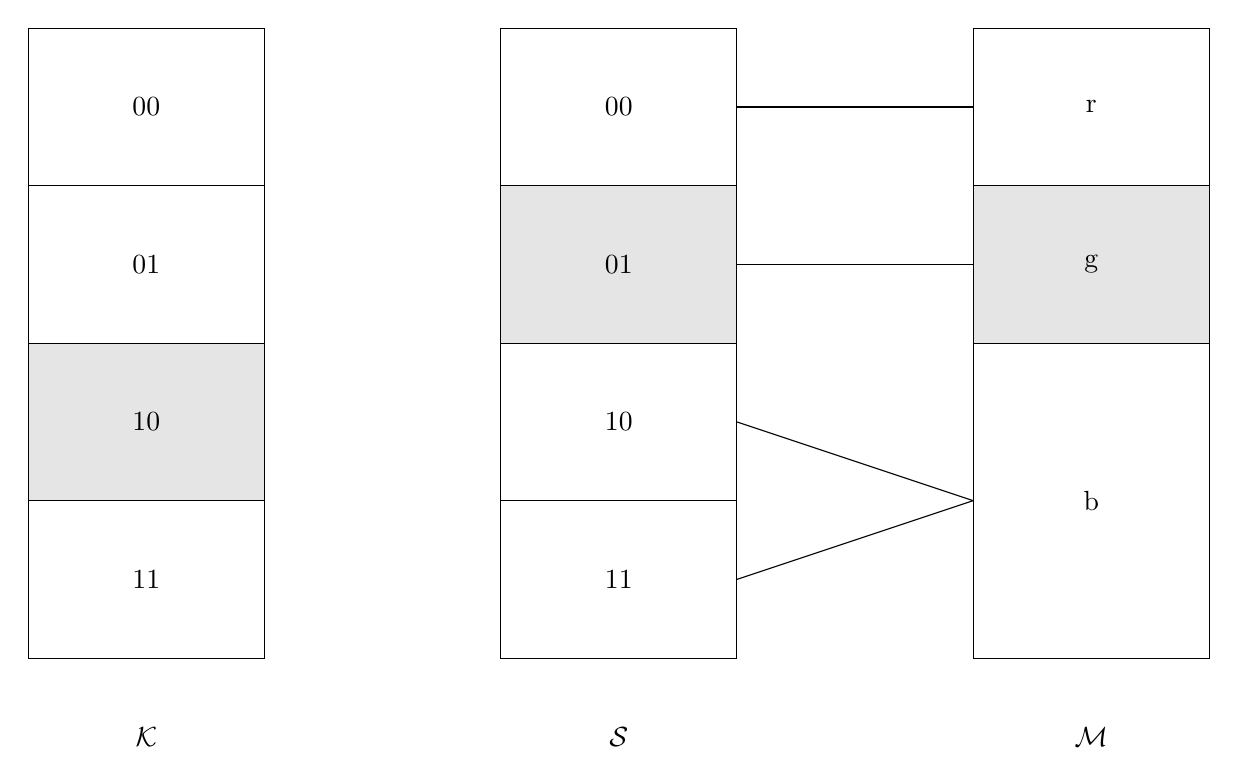
\begin{tikzpicture}
	% Linker Kasten
	\draw (1, 8) rectangle ++ (3, 2) node [midway] {$00$};
	\draw (1, 6) rectangle ++ (3, 2) node [midway] {$01$};
	\draw [fill=lightgray!40!white] (1, 4) rectangle ++ (3, 2) node [midway] {$10$};
	\draw (1, 2) rectangle ++ (3, 2) node [midway] {$11$};
	% Mittlerer Kasten
	\draw (7, 8) rectangle ++ (3, 2) node [midway] {$00$};
	\draw [fill=lightgray!40!white] (7, 6) rectangle ++ (3, 2) node [midway] {$01$};
	\draw (7, 4) rectangle ++ (3, 2) node [midway] {$10$};
	\draw (7, 2) rectangle ++ (3, 2) node [midway] {$11$};
	% Rechter Kasten
	\draw (13, 8) rectangle ++ (3, 2) node [midway] {r};
	\draw [fill=lightgray!40!white] (13, 6) rectangle ++ (3, 2) node [midway] {g};
	\draw (13, 2) rectangle ++ (3, 4) node [midway] {b};
	% Labels unten
	\node at (2.5, 1) {$\mathcal{K}$};
	\node at (8.5, 1) {$\mathcal{S}$};
	\node at (14.5, 1) {$\mathcal{M}$};
	% Linien
	\draw (10, 9) --++ (3, 0);
	\draw (10, 7) --++ (3, 0);
	\draw (10, 5) --++ (3, -1);
	\draw (10, 3) --++ (3, 1);
\end{tikzpicture}
\caption{Visualisierung unseres Beispiels}
\label{fig:Beispiel}
\end{figure}

Zur Entschlüsselung nehmen wir den Ciphertext \(C\) und XOR-verknüpfen ihn zunächst mit unserem Schlüssel \(K\) und erhalten so den Seed \(S = 11 \oplus 10 = 01\). Diesen lassen wir nun von der inversen DTE wieder auf unseren Farbanteil abbilden und erhalten wiederum grün. Ein Angreifer, dem nur \(C\) vorliegt, kann nun versuchen, unseren Farbanteil per Brute-Force zu knacken. Dazu wählt er einen Schlüssel \(K'=00\) (beispielsweise, weil dieser am häufigsten verwendet wird) und bildet \(C \oplus K' = M' = 11\). Er erhält also blau. Ebenso gut hätte er rot oder auch grün erhalten können, aber in keinem Fall kann er sicher sein, die richtige Nachricht geknackt zu haben. Seine größte Erfolgswahrscheinlichkeit erhält er also dadurch, entweder \(C\) mit dem am häufigsten verwendeten Schlüssel zu entschlüsseln oder direkt die wahrscheinlichste Nachricht \(M\) (in diesem Fall also blau) anzunehmen.

\subsection{Keine Honey Encryption-Schemata}

Um abgrenzen zu können, was Honey Encryption ausmacht, soll an dieser Stelle auf einige Verfahren eingegangen werden, die ähnlich arbeiten oder auf den ersten Blick ähnlich aussehen (die Beispiele sind entnommen aus \cite{EURO2014} und \cite{IEEE2014}).

Das erste Verfahren, das betrachtet werden soll, ist das sogenannte One Time Pad. Hierbei handelt es sich um simple XOR-Verknüpfung der Nachricht mit einem mindestens ebenso langen, zufälligen Schlüssel, der nur ein einziges Mal verwendet werden darf. Bei der Entschlüsselung lässt sich so je nach gewähltem Schlüssel jede andere (gleich lange) Nachricht mit gleicher Wahrscheinlichkeit erhalten. Bei dem One Time Pad handelt es sich jedoch nicht um ein Honey Encryption-Schema, denn erstens liefert die Entschlüsselung mit zufälligem Schlüssel nur in den wenigstens Fällen eine plausible Nachricht und zweitens werden auf jeden Fall Schlüssel hoher Entropie benötigt, Honey Encryption soll jedoch auch mit Schlüsseln geringer Entropie Sicherheit bieten.

Auch existierende AE- oder PBE-Schemata eignen sich, wie oben erklärt, nicht für die Honey Encryption, da die meisten entschlüsselten Nachrichten leicht als nicht plausibel verworfen werden können.

Als Letztes sei noch der Unterschied zu explizit gespeicherten Täuschobjekten erwähnt, wie sie beispielsweise in \cite{ACM13} verwendet werden. Bei diesen Verfahren werden neben der echten Nachricht \(n\) andere Honey Messages explizit gespeichert und (übertragen auf das hier betrachtete Gebiet) im Falle eines falschen Schlüssels bei der Entschlüsselung zurückgegeben. Im Gegensatz zur optimalen Honey Encryption ist die Erfolgswahrscheinlichkeit bei diesen Verfahren immer durch \(\frac{1}{n}\) beschränkt und unabhängig von der Entropie der Schlüsselverteilung. Außerdem haben diese Systeme einen Speicherbedarf von \(\mathcal{O}(n)\), Honey Encryption gelingt dies im Optimalfall mit einem Bedarf von \(\mathcal{O}(1)\).